\noindent
\begin{minipage}[t]{0.26\textwidth}
    \vspace{0pt}
    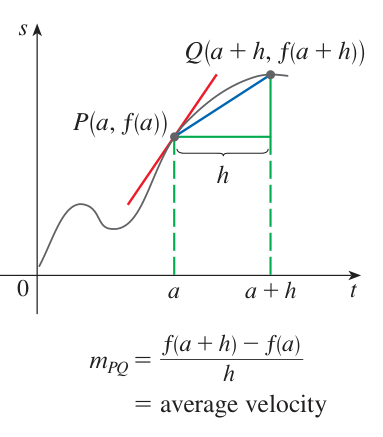
\includegraphics[width=\linewidth]{images/p0178_fig1.png}
    
    \vspace{4pt}
    \noindent\textbf{\textsf{HÌNH 6}}

    \vspace{210pt}
    \noindent\footnotesize\raggedright
    Nhắc lại từ Mục 2.1: Quãng đường (tính bằng mét) rơi sau $t$ giây là $4.9t^2$.
\end{minipage}%
\hfill
\begin{minipage}[t]{0.71\textwidth}
    \vspace{0pt}
    Vận tốc trung bình trong khoảng thời gian này là
    \[
    \text{vận tốc trung bình} = \frac{\text{độ dời}}{\text{thời gian}} = \frac{f(a+h) - f(a)}{h}
    \]
    chính là hệ số góc của cát tuyến $PQ$ trong Hình 6.

    Bây giờ giả sử chúng ta tính các vận tốc trung bình trên các khoảng thời gian $[a, a + h]$ ngày càng ngắn hơn. Nói cách khác, ta cho $h$ dần tới $0$. Tương tự như trong ví dụ quả bóng rơi, ta định nghĩa \textbf{vận tốc} (hay \textbf{vận tốc tức thời}) $v(a)$ tại thời điểm $t = a$ là giới hạn của các vận tốc trung bình này.

    \vspace{3pt}
    \begin{definitionbox}
        \noindent
        \tcbox[colback=white,colframe=stewartred,arc=0mm,boxrule=0.8pt,top=1.5pt,bottom=1.5pt,left=3.5pt,right=3.5pt,on line]{\textbf{\color{stewartred}\textsf{3}}}\hspace{0.5em}\textbf{\color{stewartred}\textsf{Định nghĩa}}\hspace{0.8em}\textbf{Vận tốc tức thời} của một vật có hàm vị trí $f(t)$ tại thời điểm $t = a$ là
        \setlength{\abovedisplayskip}{6pt}
        \setlength{\belowdisplayskip}{6pt}
        \[
        v(a) = \lim_{h \to 0} \frac{f(a+h) - f(a)}{h}
        \]
        \noindent miễn là giới hạn này tồn tại.
    \end{definitionbox}
    \vspace{3pt}

    Điều này có nghĩa là vận tốc tại thời điểm $t = a$ bằng với hệ số góc của tiếp tuyến tại $P$ (so sánh Phương trình 2 và biểu thức trong Định nghĩa 3).

    Bây giờ khi đã biết cách tính giới hạn, chúng ta hãy xem xét lại bài toán quả bóng rơi từ Mục 2.1.

    \vspace{6pt}
    \noindent\textbf{\textsf{\color{stewartcyan}VÍ DỤ 3}}\hspace{1em}Giả sử một quả bóng được thả rơi từ đài quan sát phía trên của Tháp CN, cách mặt đất $450\text{ m}$.
    \begin{enumerate}[label=\textbf{(\alph*)}, itemsep=1pt, topsep=2pt, leftmargin=1.5em]
        \item Vận tốc của quả bóng sau $5$ giây là bao nhiêu?
        \item Quả bóng chuyển động nhanh như thế nào khi chạm đất?
    \end{enumerate}

    \vspace{4pt}
    \noindent\textbf{\textsf{\color{stewartcyan}LỜI GIẢI}}\hspace{1em}Vì bài toán yêu cầu hai vận tốc khác nhau, nên sẽ hiệu quả hơn nếu bắt đầu bằng cách tìm vận tốc tại một thời điểm tổng quát $t = a$. Sử dụng phương trình chuyển động $s = f(t) = 4.9t^2$, ta có
    \begin{align*}
    v(a) &= \lim_{h \to 0} \frac{f(a+h) - f(a)}{h} = \lim_{h \to 0} \frac{4.9(a+h)^2 - 4.9a^2}{h} \\[4pt]
    &= \lim_{h \to 0} \frac{4.9(a^2 + 2ah + h^2 - a^2)}{h} = \lim_{h \to 0} \frac{4.9(2ah + h^2)}{h} \\[4pt]
    &= \lim_{h \to 0} \frac{4.9h(2a + h)}{h} = \lim_{h \to 0} 4.9(2a + h) = 9.8a
    \end{align*}

    \noindent\textbf{(a)} Vận tốc sau $5$ giây là $v(5) = (9.8)(5) = 49\text{ m/s}$.

    \vspace{2pt}
    \noindent\textbf{(b)} Vì đài quan sát cách mặt đất $450\text{ m}$, quả bóng sẽ chạm đất tại thời điểm $t$ khi $s(t) = 450$, tức là
    \[
    4.9t^2 = 450
    \]
    Từ đó suy ra
    \[
    t^2 = \frac{450}{4.9} \qquad \text{và} \qquad t = \sqrt{\frac{450}{4.9}} \approx 9.6\text{ s}
    \]
\end{minipage}
